\part{The method}\label{part:method}

\section{Purpose and how to read this document}

This document describes, from the transport equation upward, a hybrid method that computes
continuous-energy (CE) eigenvalue solutions by \emph{correcting} a cheap multigroup (MG) random-ray
solution with Monte Carlo. It has four parts.

\begin{enumerate}
\item \textbf{The method} (this part): the mathematics and the intuition of every stage, the
  estimators grouped into classes, why each is unbiased, and what sets its variance and cost.
\item \textbf{Results}: every test that has been run, with its setup, what it shows, and the first
  end-to-end measurement against a CE Monte Carlo reference, including a figure of merit and its
  projection after optimization.
\item \textbf{Nuclear data}: the reactions, how they are represented and stored, how they shape
  real spectra, how OpenMC samples each one, and how each one constrains this method.
\item \textbf{Implementation}: the structure of the code inside OpenMC, its data containers and
  algorithms, and the performance consequences of each design choice.
\end{enumerate}

Mathematics comes first in each section, then pseudocode, then the implementation. Boxes labelled
\emph{Intuition} give the physical picture; boxes with a title state results that later sections
rely on. The notation is collected in Appendix~\ref{app:notation}. The code lives on the
\code{rmc} branch of an OpenMC fork, in \code{include/openmc/rmc}, \code{src/rmc},
\code{openmc/lib/rmc.py} and \code{examples/rmc}; the version-controlled methods chapter is
\code{docs/source/methods/rmc.rst} and the development log \code{docs/source/devguide/rmc.rst}.

\section{Transport background and notation}\label{sec:background}

\subsection{The phase space and the flux}

A neutron is described by its position $\vr$, its kinetic energy $E$ and its direction of flight
$\vO$ (a unit vector). The \textbf{angular flux} $\psi(\vr,E,\vO)$ is the neutron density times
speed, per unit volume, energy and solid angle; the \textbf{scalar flux} is
$\phi(\vr,E)=\int_{4\pi}\psi\dd\Omega$. A reaction rate density is a cross section times the flux:
$\Sigma_x(\vr,E)\,\phi(\vr,E)$ reactions per unit volume, time and energy. The macroscopic cross
section $\Sigma_x=\sum_i N_i\sigma_{x,i}$ sums the microscopic cross sections $\sigma_{x,i}$ of the
nuclides $i$ in the material, weighted by their atom densities $N_i$.

\subsection{The emission density}

The quantity at the centre of this method is not the flux but the \textbf{emission density}
$Q(\vr,E,\vO)$: the rate at which neutrons \emph{leave} collisions (or are born) at a point of phase
space. It has two parts, which we keep separate and call \emph{tags}:
\begin{align}
Q_s(\vr,E,\vO) &= \int\!\!\int \Sigma_s(\vr; E'\to E, \vO'\to\vO)\,\psi(\vr,E',\vO')\dd E'\dd\Omega',
\label{eq:Qs}\\
Q_f(\vr,E,\vO) &= \frac{1}{4\pi}\,\frac{1}{k}\int \chi(\vr; E\mid E')\,\nu\Sigma_f(\vr,E')\,\phi(\vr,E')\dd E'.
\label{eq:Qf}
\end{align}
$\Sigma_s(E'\to E,\vO'\to\vO)$ is the double-differential \emph{production} kernel of every
non-fission reaction with outgoing neutrons (elastic scattering, inelastic scattering,
$(n,2n)$, \dots), including their multiplicities; $\chi(E\mid E')$ is the fission spectrum and
$\nu\Sigma_f$ the fission neutron production. Fission emission is isotropic. The factor $1/k$ is the
eigenvalue normalization: in the $k$-eigenvalue problem the number of fission neutrons is divided by
$k$ so that a steady state exists.

\subsection{Two operators: flight and collision}

Write the transport equation as
\begin{equation}
\vO\cdot\nabla\psi + \Sigma_t\psi = Q_s + Q_f .
\end{equation}
Given an emission density $Q$, the flux it produces before any further collision is obtained by
integrating along the characteristic (the straight line) ending at $(\vr,\vO)$:
\begin{equation}\label{eq:G}
\psi(\vr,E,\vO) = (\G Q)(\vr,E,\vO) = \int_0^\infty e^{-\tau(\vr,\vr-s\vO;E)}\;Q(\vr-s\vO,E,\vO)\dd s ,
\end{equation}
where $\tau$ is the optical depth along the path. $\G$ is the \textbf{flight} (or first-flight, or
streaming) operator. The \textbf{collision} operator $\mathcal P(k)$ turns a flux into the next emission
density through equations \eqref{eq:Qs}--\eqref{eq:Qf}. Their product
\begin{equation}
\B(k)=\mathcal P(k)\,\G
\end{equation}
maps one \emph{generation} of emission to the next: where neutrons leave collisions now, to where
they leave their next collision. The CE eigenvalue problem is the fixed point
\begin{equation}
Q=\B(k)\,Q, \qquad \text{with } \langle\nu\Sigma_f,\G Q\rangle\text{ fixed},
\end{equation}
and $k$ is the value for which it has a positive solution. Analog Monte Carlo is the stochastic
version of iterating $\B$: each history samples a flight and a collision, again and again.

\begin{intuition}
An emission density is a ``where neutrons start'' map. Applying $\G$ smears each start along its
direction of flight with exponential attenuation; applying $\mathcal P$ turns the resulting flux
into new starts by scattering (which mostly lowers the energy) and fission (which restarts
neutrons at MeV energies). One power of $\B$ is one link in every neutron's chain of collisions.
\end{intuition}

\subsection{Monte Carlo estimators, variance and figure of merit}

An \textbf{estimator} is a random variable whose expectation is the quantity sought; it is
\textbf{unbiased} if the equality is exact. If one sample has variance $V$ and costs $C$ seconds, the
average of $N$ samples has variance $V/N$ and costs $NC$, so reaching a root-mean-square error
$\varepsilon$ costs $VC/\varepsilon^2$. The \textbf{figure of merit} $\mathrm{FOM}=1/(\sigma^2T)$ is
the inverse of $VC$: halving the variance at equal time doubles it. Every comparison in this document
is ultimately a comparison of $VC$.

A set of weighted particles $\{(x_i,w_i)\}$ with $x_i=(\vr_i,E_i,\vO_i)$ \emph{represents} a
(signed) measure $\mu$ if $\E[\sum_iw_iv(x_i)]=\int v\dd\mu$ for every response $v$. A particle bank
is a random object whose average, tested against any response, is the source it stands for. Its
\textbf{absolute weight} $\Wabs=\sum_i|w_i|$ is what sets the noise of every tally made from it: a
bank of $+1$ and $-1$ particles with zero net weight still carries noise of size $\Wabs$.

\section{The idea: a deterministic field plus a Monte Carlo correction}\label{sec:idea}

\subsection{Splitting the emission density}

A multigroup random-ray solve gives, cheaply and with little noise, an emission density that is
\emph{almost} right. Call it the \textbf{field} $Q^F$. The CE truth differs from it by a small signed
correction:
\begin{equation}
Q = Q^F + \delta Q .
\end{equation}
The correction is carried by a bank of signed Monte Carlo particles. One generation updates both
parts:
\begin{equation}\label{eq:update}
Q_{n+1} = \B(k_n)\,Q_n = \underbrace{\B Q^F_n - F_{n+1}}_{\text{residual }\widehat R_n} + F_{n+1}
 + \underbrace{\B\,\delta Q_n}_{\text{flights}} .
\end{equation}
$F_{n+1}$ is the part of the new emission that is kept in the field (with a frozen shape, the same
MG emission times amplitudes); the rest goes to the bank. The bank's update has two pieces:
\begin{itemize}
\item the \textbf{residual} $\B Q^F - F$: the CE emission the field produces in one generation,
  minus what the field already says. If the field were the exact CE solution this would be zero;
  for a good MG field it is small and signed;
\item the \textbf{flights}: the existing correction particles carried one generation forward by
  analog CE transport.
\end{itemize}

\begin{figure}[t]\centering
\begin{tikzpicture}[node distance=7mm and 10mm]
\node[box,minimum width=33mm] (rr) {Random ray (MG)\\ converged once};
\node[box,right=of rr,minimum width=33mm] (field) {Field $Q^F=a\cdot\Qmg$\\ lifted to CE by $h_t(E)$};
\node[box,below=12mm of field,minimum width=33mm] (res) {Residual\\ $\B Q^F - F_{n+1}$\\ \footnotesize backward CE traces};
\node[box,right=14mm of res,minimum width=30mm] (fl) {Flights\\ $\B\,\delta Q_n$\\ \footnotesize one CE collision};
\node[box,below=10mm of res,xshift=19mm,minimum width=40mm] (cand) {Candidate bank $\delta Q^\ast_{n+1}$};
\node[box,below=8mm of cand,minimum width=40mm] (canc) {Cancellation\\ \footnotesize pooling, netting};
\node[box,below=8mm of canc,minimum width=40mm] (norm) {$f_n$, $k_{n+1}$, scaling,\\ resampling};
\node[box,left=14mm of norm,minimum width=30mm] (tally) {Correction tally\\ field + bank};
\draw[arr] (rr)--(field);
\draw[arr] (field)--(res);
\draw[arr] (res)--(cand);
\draw[arr] (fl)--(cand);
\draw[arr] (cand)--(canc);
\draw[arr] (canc)--(norm);
\draw[arr] (norm.east) -- ++(18mm,0) |- node[note,pos=0.25,right]{bank $\delta Q_{n+1}$} (fl.east);
\draw[arr] (norm.west) -- (tally.east);
\draw[arr] (norm.south) -- ++(0,-5mm) -| node[note,pos=0.2,below]{amplitudes $a_{n+1}$} ([xshift=-25mm]field.west) -- (field.west);
\end{tikzpicture}
\caption{One generation of the method. The field is a multigroup solution lifted to continuous
energy; the bank of signed CE particles carries what the field misses. Everything is driven by two
CE kernels: backward traces (residual) and forward one-collision flights.}\label{fig:overview}
\end{figure}

Figure~\ref{fig:overview} shows the loop. Its correctness is a one-line argument:
\begin{keybox}[Why the iteration is right]
If the residual and the flights are unbiased estimates of $\B Q^F_n-F_{n+1}$ and $\B\,\delta Q_n$,
then $\E[F_{n+1}+\delta Q_{n+1}]=\B(k_n)(Q^F_n+\E\delta Q_n)$: in expectation the method applies
exactly one CE generation per step. Everything the field gets wrong (group structure, flat sources,
P$_0$ scattering, self-shielding) is corrected by the bank, at a cost set by how much the field gets
wrong.
\end{keybox}

\subsection{Why it might pay off}

Analog Monte Carlo spends its particles on the whole emission density. This method spends them on
the residual, whose size is the field's error. If the residual can be estimated with noise
proportional to its own size, and if the bank stays small, the Monte Carlo variance scales with the
field's error rather than with the solution, as in multilevel Monte Carlo. Two things stand in the way,
and much of this document is about them:
\begin{enumerate}
\item \textbf{The residual's estimator must have residual-scale noise.} The difference
  $\B Q^F-F$ is small, but each of its terms is production-scale. Unless the two terms are evaluated
  so that their noise cancels, the estimate is as noisy as the production itself
  (Section~\ref{sec:residual}).
\item \textbf{Signed weights must cancel.} Particles never interact, so a positive and a negative
  particle at the same place do not annihilate by themselves; without cancellation $\Wabs$ grows
  with each generation (Section~\ref{sec:cancellation}).
\end{enumerate}

\section{Random ray in one section}\label{sec:randomray}

The field comes from OpenMC's random-ray solver, a stochastic method of characteristics. It solves
the MG transport equation with a flat (constant) emission in each source region:
\begin{enumerate}
\item \textbf{Rays.} Each batch launches rays from uniform points in a box with isotropic directions.
  A ray first travels a \emph{dead} length without tallying, so that its angular flux forgets its
  arbitrary starting value, then an \emph{active} length.
\item \textbf{Attenuation.} Along a segment of length $\ell$ in region $R$, with the region's MG source
  $Q_{R,g}/4\pi$, the angular flux changes exactly as
  $\psi_{out}=\psi_{in}e^{-\Sigma_{t,g}\ell}+\frac{Q_{R,g}}{4\pi\Sigma_{t,g}}(1-e^{-\Sigma_{t,g}\ell})$,
  and the segment's contribution to the region's scalar flux is the average of $\psi$ over it, times
  $\ell$.
\item \textbf{Region flux.} Summing over segments and dividing by the total track length per unit
  volume gives $\bar\phi_{R,g}$; a power iteration updates $Q$ and $k$ from it.
\end{enumerate}
The method is \emph{biased} by the flat-source approximation and the multigroup cross sections, and
noisy because the rays are random; averaging many batches removes the noise but not the
discretization. That discretization error is exactly what the residual measures. In this method
random ray is used twice: once, to produce the field; and, optionally, every generation as a
\emph{sweep} whose segments serve as quadrature directions and whose region emission
$\hat Q$ is the MG update of the field (tandem estimators).

\begin{figure}[t]\centering
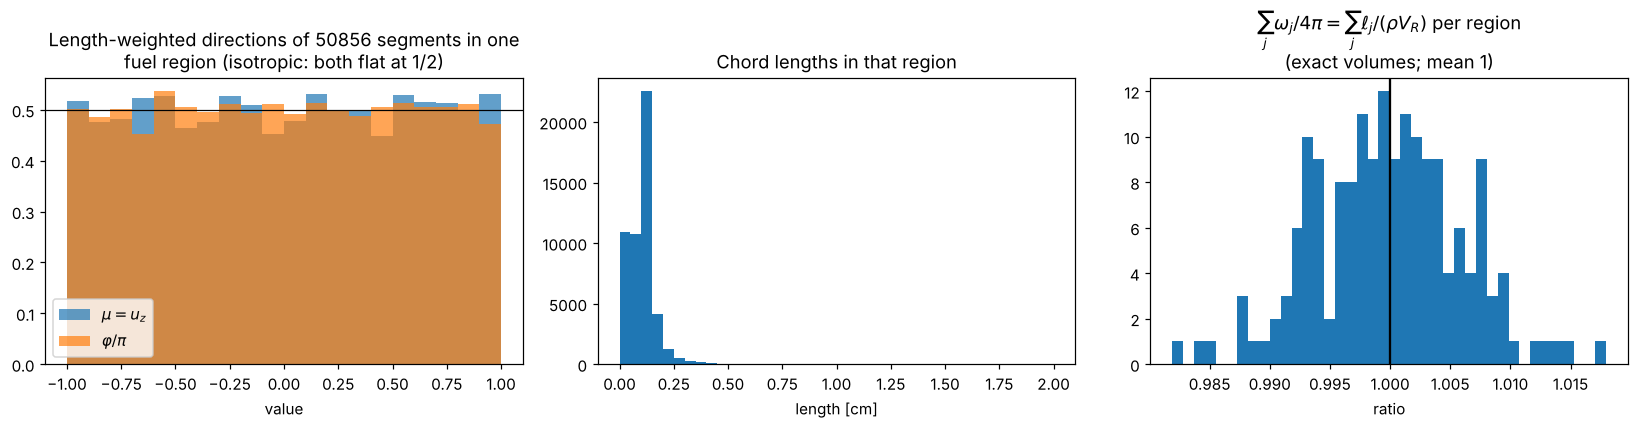
\includegraphics[width=0.8\textwidth]{figures/segments.png}
\caption{Segments of a random-ray sweep crossing one source region: each carries a direction, a chord
length and a chord-averaged MG angular flux; with weights $\omega_j=4\pi\ell_j/(\rho V_R)$ they form an
unbiased quadrature of the angular integral at points of the region.}\label{fig:segments}
\end{figure}

\section{The frozen field}\label{sec:field}

\subsection{From random ray to a continuous-energy emission density}

The random-ray solve (OpenMC's own solver) uses flat sources in \emph{source regions} $R$ (a cell, or
a cell cut by a mesh) and $G$ energy groups. It returns region-group scalar fluxes $\bar\phi_{R,g}$,
from which the MG emission densities per unit volume (integrated over angle and group) follow:
\begin{equation}
Q_{s,R,g}=d_R\sum_{g'}\nu\Sigma_{s,m}(g'\to g)\,\bar\phi_{R,g'},\qquad
Q_{f,R,g}=d_R\,\frac{\chi_{m,g}}{k^{\mathrm{MG}}}\sum_{g'}\nu\Sigma_{f,m,g'}\,\bar\phi_{R,g'},
\end{equation}
with $m$ the region's material and $d_R$ its density multiplier. A CE method needs an emission at
every energy, so each group is \textbf{lifted} by a within-group shape:
\begin{equation}\label{eq:field}
\Qmg_t(\vr,E,\vO)=\frac{1}{4\pi}\,Q_{t,R(\vr),g(E)}\,h_{t,m,g}(E),\qquad \int_g h_{t,m,g}\dd E=1 .
\end{equation}
The lifts $h_s,h_f$ (and a flux shape $h^\phi$ used only for proposals) are histograms on a fine
energy grid, tallied once from a short CE run of the same material. The field is a
\emph{definition}: any choice of lifts gives a valid field, and a better choice only makes the
residual smaller. The amplitudes $a=(a_s,a_f)$ scale the two tags: $Q^F=a_s\Qmg_s+a_f\Qmg_f$.

\begin{figure}[t]\centering
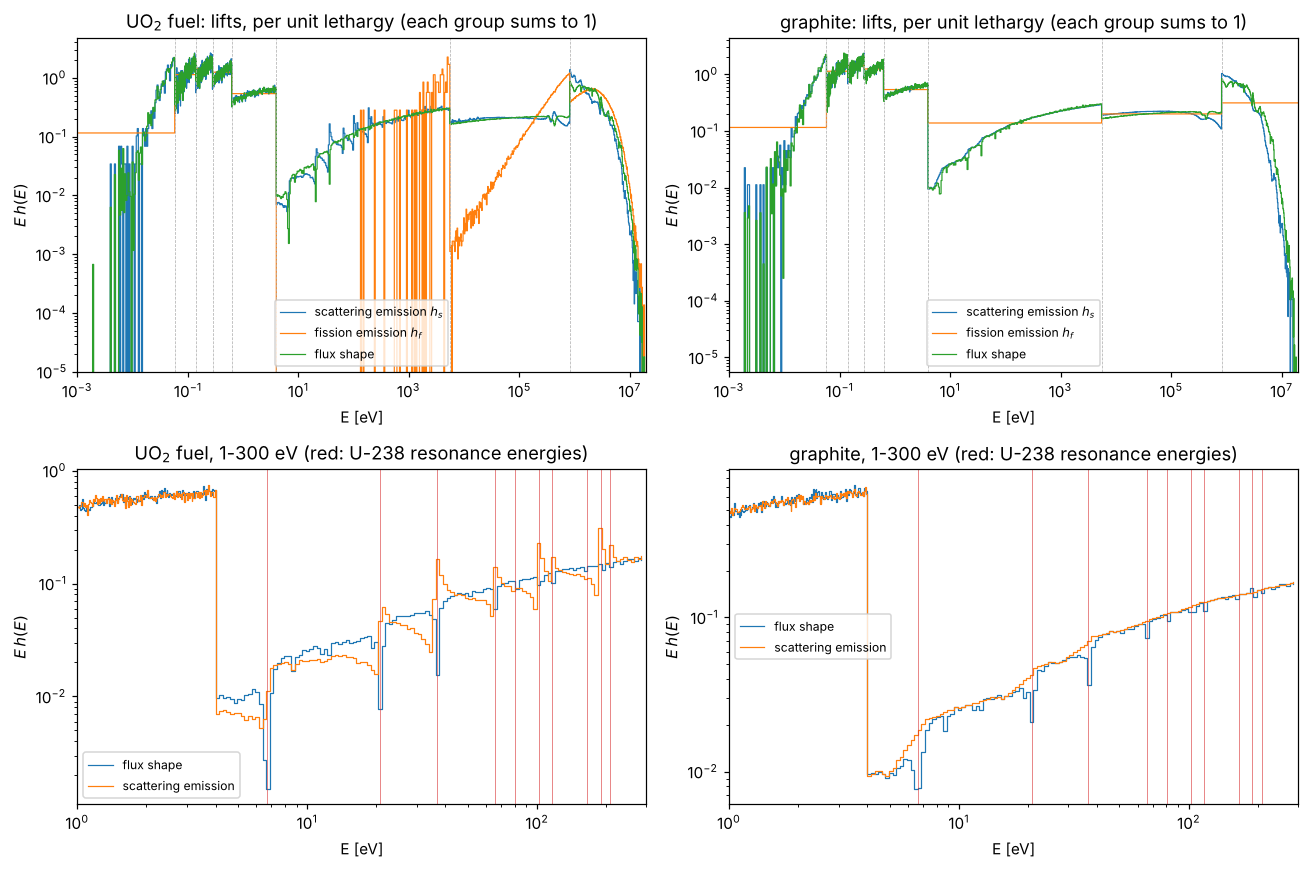
\includegraphics[width=0.92\textwidth]{figures/lifts.png}
\caption{Lifts of the graphite pincell: within-group shapes of the scattering emission, fission
emission and flux in the fuel and the graphite, on the fine grid (200 bins per group). The lifts carry
the resonance structure and the fission spectrum that eight groups cannot.}\label{fig:lifts}
\end{figure}

\subsection{Normalization and volumes}

The field is scaled to unit MG fission production, $\langle 1,\Qmg_f\rangle=\sum_RV_R\sum_gQ_{f,R,g}=
1/k^{\mathrm{MG}}$, so the iteration starts from $a_0=(1,1)$ and $k_0=k^{\mathrm{MG}}$. Region
volumes $V_R$ enter the normalization, the field's masses, the sweep weights and every exact integral
of the field. OpenMC's random ray can be given \emph{prescribed} volumes; with the exact volumes of the
source regions (each mesh voxel cut by the pin surface in closed form) the field and every reference
integral use the true geometry. With point-sampled volumes the small regions at the pin surface carry
a few per cent of error, which appears as apparent bias in any test that integrates the field exactly
(Section~\ref{sec:res:controlled}).

\section{The backward characteristic}\label{sec:backward}

\subsection{What is computed}

The residual needs the CE flux that the field produces at a chosen point, direction and energy:
equation~\eqref{eq:G} with $Q=Q^F$. Along the backward path $\vr(s)=\vr^\star-s\vO'$ (folded through
reflecting boundaries) the path crosses segments $k$ of length $\ell_k$, each in one region and one
material. With the field flat in a region and CE cross sections constant along a segment,
\begin{equation}\label{eq:psi}
\psi(\vr^\star,E',\vO')=\sum_k e^{-\tau_k(E')}\,q_k(E')\,
\frac{1-e^{-\Sigma_{t,k}(E')\ell_k}}{\Sigma_{t,k}(E')},\qquad q_k(E')=Q^F(R_k,E'),
\end{equation}
where $\tau_k$ is the optical depth from $\vr^\star$ to the near end of segment $k$. Two choices make
this cheap: the geometry is traced \emph{once} per direction and reused for every energy requested
on it, and the trace is extended lazily in chunks only while some energy is still alive.

\begin{figure}[t]\centering
\begin{tikzpicture}[scale=1.0]
\draw[thick] (0,0) rectangle (9,3.2);
\foreach \x in {1.5,3,4.5,6,7.5} \draw[gray!50] (\x,0)--(\x,3.2);
\fill[accred!15] (4.5,1.6) circle (1.0);
\draw[accred!70] (4.5,1.6) circle (1.0);
\node[accred] at (4.5,2.85) {\footnotesize fuel};
\fill[headblue] (6.8,1.9) circle (2pt) node[above right] {$\vr^\star$};
\draw[-{Stealth},very thick,headblue] (6.8,1.9) -- (7.9,2.3) node[above] {$\vO'$};
\draw[thick,dashed,headblue] (6.8,1.9) -- (1.6,0.0);
\draw[thick,dashed,headblue] (1.6,0.0) -- (0,0.58);
\node[note] at (2.2,2.5) {backward path $\vr^\star-s\vO'$\\ (reflects at the boundary)};
\foreach \p/\l in {{(5.9,1.57)}/1,{(4.9,1.20)}/2,{(3.8,0.80)}/3,{(2.6,0.37)}/4} \node[circle,fill=white,draw=headblue,inner sep=0.8pt,font=\tiny] at \p {\l};
\draw[decorate,decoration={brace,amplitude=4pt,mirror}] (0,-0.2) -- (9,-0.2) node[midway,below=4pt,note] {each segment $k$: length $\ell_k$, material, region $R_k$; flat field $q_k(E')$ and CE $\Sigma_{t,k}(E')$};
\end{tikzpicture}
\caption{The backward characteristic from a destination $\vr^\star$ against the incident direction
$\vO'$: one geometric trace (here crossing a source-region mesh, the fuel pin and a reflecting face)
serves every incident energy requested on it.}\label{fig:backward}
\end{figure}

\subsection{Tails: why roulette is unbiased}

In a reflective problem the path never ends; it must be cut. Cutting at a fixed length biases the
estimate. \textbf{Roulette} does not: when the transmission $T=e^{-\tau}$ along the path falls below a
threshold $T_c$, the path continues with probability $T/T_c$ and with $T$ reset to $T_c$, or stops.
\begin{proposition}
For any $T_c>0$ the roulette estimate of \eqref{eq:psi} has the same expectation as the infinite sum.
\end{proposition}
\begin{proof}
Consider the contribution of the remaining path beyond the point where $T<T_c$ is first reached; it
is $T\cdot S$ with $S$ the (unattenuated-from-here) remainder. Roulette returns $T_c\,S'$ with
probability $T/T_c$ and $0$ otherwise, where $S'$ is the same construction applied recursively. By
induction $\E S'=S$, so the expectation is $(T/T_c)\,T_c\,S=T\,S$.
\end{proof}
The threshold therefore trades variance against cost and never moves the mean.
Figure~\ref{fig:backward_tails} compares the three tails implemented: vacuum (exact, only where paths
leave), roulette, and a fixed dead length (biased, no noise).

\begin{figure}[t]\centering
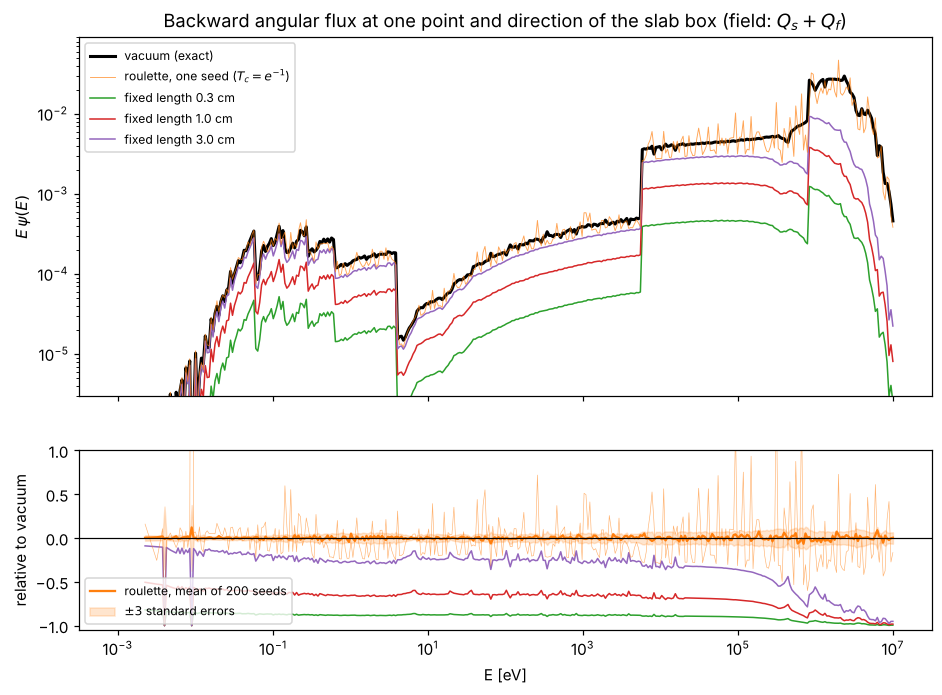
\includegraphics[width=0.85\textwidth]{figures/backward_tails.png}
\caption{Backward $\psi$ in the infinite medium with the three tails against the closed form
$q(E')/\Sigma_t(E')$. Roulette is unbiased at every threshold; its noise appears where the mean free
path is long compared with the geometry.}\label{fig:backward_tails}
\end{figure}

\section{Production at a common output}\label{sec:production}

\subsection{The problem}

The residual compares the CE emission produced by the field with the field itself \emph{at the same
outgoing state} $(\vr^\star,E,\vO)$. The CE emission there is the integral \eqref{eq:Qs}--\eqref{eq:Qf}
over incident energy and direction, with the backward $\psi$ as the incident flux. Over incident
directions we use a quadrature or random directions; over incident energy there are two very
different possibilities, which give the two \emph{routes} of every reaction.

\subsection{The evaluator route: densities}

If the production kernel has a known density in the outgoing variables, we can evaluate it at the
chosen output. For \textbf{fission}, emission is isotropic and the outgoing energy has density
$\chi(E\mid E')$; with one incident energy drawn from a proposal $g(E')$,
\begin{equation}\label{eq:fission_eval}
\int\!\!\int \frac{\chi(E\mid E')\nu\Sigma_f(E')}{4\pi k}\psi(E',\vO')\dd E'\dd\Omega'
\approx \sum_j\omega_j\,\frac{\nu\Sigma_f(E'_j)\,\chi(E\mid E'_j)\,\psi(\vr^\star,E'_j,\vO'_j)}{4\pi k\,g(E'_j)} .
\end{equation}
OpenMC can only sample $\chi$; the evaluator implements the density of exactly what OpenMC's sampler
does, including the interpolation between tabulated incident energies and the rescaling of outgoing
energies to interpolated endpoints (Section~\ref{sec:nd:openmc}).

For \textbf{elastic scattering off a stationary target} of mass ratio $A>1$, energy and angle are tied
by two-body kinematics: an incident neutron at $E'$ deflected by laboratory cosine
$\mu_0=\vO'\cdot\vO$ leaves with $E=E'\gamma_A(\mu_0)$, where
\begin{equation}
\gamma_A(\mu_0)=\left(\frac{\mu_0+\sqrt{A^2-1+\mu_0^2}}{A+1}\right)^2 .
\end{equation}
Given the output $(E,\vO)$ and an incident direction, there is exactly one incident energy that can
produce it, the \textbf{image} $E'=E/\gamma_A(\mu_0)$. The energy integral collapses onto it:
\begin{equation}\label{eq:elastic_image}
\int\K^{el}\psi\dd E'=\sum_iN_i\,\sigma_{el,i}(E'_i)\,
\frac{p_{lab,i}(\mu_0\mid E'_i)}{2\pi\,\gamma_{A_i}(\mu_0)}\,\psi(\vr^\star,E'_i,\vO'),
\qquad p_{lab}=p_{cm}(\mu_{cm}(\mu_0))\left|\frac{\dd\mu_{cm}}{\dd\mu_0}\right| .
\end{equation}
The Jacobian $1/\gamma$ converts the delta function in energy; $p_{lab}$ converts the tabulated
centre-of-mass angular distribution to the laboratory. No incident energy is sampled at all, so the
elastic evaluator has no energy-integration noise; its noise is in the incident direction.

\begin{figure}[t]\centering
\begin{tikzpicture}[scale=1.1]
\draw[-{Stealth},thick] (0,0) -- (4,0) node[right] {$\mathbf v'$ (lab)};
\draw[-{Stealth},thick,headblue] (0,0) -- (2.2,0) node[below,pos=0.6] {$\mathbf V_{cm}$};
\draw[dashed,gray] (2.2,0) circle (1.6);
\draw[-{Stealth},thick,accred] (2.2,0) -- ({2.2+1.6*cos(60)},{1.6*sin(60)}) node[right] {$\mathbf v_{cm}$};
\draw[-{Stealth},very thick,accgreen] (0,0) -- ({2.2+1.6*cos(60)},{1.6*sin(60)}) node[above left,pos=0.6] {$\mathbf v$};
\draw (0.8,0) arc (0:{atan(1.6*sin(60)/(2.2+1.6*cos(60)))}:0.8) node[midway,right,font=\footnotesize] {$\mu_0$};
\draw ({2.2+0.45},0) arc (0:60:0.45) node[midway,right,font=\footnotesize] {$\mu_{cm}$};
\node[note,align=left] at (7.6,0.9) {Two-body kinematics: fixing the outgoing\\ lab direction and the incident
direction fixes\\ $\mu_0$, hence $\mu_{cm}$ and $E/E'=\gamma_A(\mu_0)$.\\ Fixing also $E$ fixes $E'$: the image.};
\end{tikzpicture}
\caption{Elastic scattering off a stationary target in velocity space. The centre-of-mass velocity
$\mathbf V_{cm}=\mathbf v'/(A+1)$; in the CM frame the neutron speed is unchanged and only its direction
is sampled. The lab outgoing velocity lies on the dashed circle.}\label{fig:kinematics}
\end{figure}

\subsection{The sampler route: OpenMC's own collision routines}

Every other channel (elastic scattering off a moving target, S($\alpha,\beta$), inelastic levels and
continuum, $(n,xn)$) is handled by OpenMC's own collision routine: draw $E'$ from $g$, choose a
sampler-route channel with probability proportional to its production
$\Sigma^{samp}_{\mathcal P}(E')$, call the routine on a scratch particle, and keep the outgoing state
as a new particle with weight
\begin{equation}\label{eq:sampler_weight}
c=\omega_j\,\frac{\Sigma^{samp}_{\mathcal P}(E')\,\psi(\vr^\star,E',\vO'_j)}{g(E')} .
\end{equation}
Its expectation is the sampler-route production at its own (random) outgoing state: correct by
construction for every law OpenMC supports. The price is that its state is \emph{not} the destination's
outgoing state, which matters for the residual (Section~\ref{sec:lowterm}).

\begin{keybox}[The channel registry]
Every reaction with outgoing neutrons is a \emph{channel} (nuclide, reaction, tag). At every incident
energy each channel is on exactly one route, so evaluator plus sampler production equals the tag's
total production and nothing is counted twice. Capture belongs to no channel but stays in $\Sigma_t$.
Stationary elastic and fission are on the evaluator route by default; with \code{all\_sampler} every
channel goes to the sampler route and the estimator needs no density at all.
\end{keybox}

\section{The residual estimator}\label{sec:residual}

\subsection{One residual sample}

The residual of tag $t$ is $R_t=\K_tQ^F-b_t\Qmg_t$ with $\K_t=\mathcal P_t\G$ the CE production of
tag $t$. One sample (Figure~\ref{fig:sample}):
\begin{enumerate}
\item \textbf{Destination.} $\vr^\star$ uniform in the field's box (or in regions weighted by volume
  or emission); locate its region $R$ and material $m$.
\item \textbf{Outgoing state.} $\vO$ isotropic, $E$ from a mixture of the region's emission spectrum
  and a log-uniform component (so that the support covers every $E$ where the residual can be
  nonzero). The sample's density is $\varrho=\pi(\vr^\star)\,p(E)/4\pi$.
\item \textbf{Directions.} $J$ incident directions $\vO'_j$ with weights $\omega_j$: a spherical
  Fibonacci set under a uniformly random rotation ($\omega_j=4\pi/J$), or the segments of a random-ray
  sweep crossing $R$.
\item \textbf{Traces.} One backward trace per direction; on it the incident energies of every
  evaluator (images for elastic, a drawn $E'$ for fission) and the sampler route's $K$ energies.
\item \textbf{Record.} The density-branch record stores the CE production at $(E,\vO)$ per source
  tag, $C_y$, the MG control $M_y$ and its restored mean $R_y$ (below), and the field value
  $U=\Qmg_t(\vr^\star,E)$. Sampler particles are separate records with their own state.
\end{enumerate}
The weight of a density record, for amplitudes $a,b$, eigenvalue $k$, control coefficient $c$ and
mixing $\lambda$, is
\begin{equation}\label{eq:weight}
w=\frac{1}{N\varrho}\Big\{\frac{\sum_ya_y\,(C_y-cM_y+cR_y)}{k^{[t=f]}}-b_t\big[(1-\lambda)U+
\lambda\,\tfrac{\sum_ya_yR_y}{k^{[t=f]}}\big]\Big\},
\end{equation}
and a sampler particle has $w=(\sum_ya_yC_y+Z)/(k^{[t=f]}N\varrho)$. The records do not depend on
$(a,b,k,c,\lambda)$: one set of samples serves every value, so variants can be compared on identical
random numbers and residuals can be generated ahead of the generation that uses them.

\begin{figure}[t]\centering
\begin{tikzpicture}[scale=1]
\fill[headblue] (0,0) circle (2.5pt) node[below left] {$\vr^\star$};
\foreach \a/\l in {20/1,75/2,140/3,200/4,260/5,320/6} {
  \draw[thick,headblue!70,dashed] (0,0) -- ({2.4*cos(\a)},{2.4*sin(\a)});
  \node[font=\tiny,headblue] at ({2.65*cos(\a)},{2.65*sin(\a)}) {$\vO'_{\l}$};
}
\draw[-{Stealth},very thick,accred] (0,0) -- (1.3,0.35) node[right,font=\footnotesize] {$(E,\vO)$: record};
\draw[-{Stealth},thick,accgreen] (0,0) -- (-0.9,1.0) node[left,font=\footnotesize] {sampler particle};
\draw[-{Stealth},thick,accgreen] (0,0) -- (0.4,-1.2) node[below,font=\footnotesize] {sampler particle};
\node[note,align=left,anchor=west] at (3.6,1.0) {\textbf{Density branch}: at the chosen output $(E,\vO)$\\
CE production $C$ from images / $\chi$ on every $\vO'_j$,\\ minus the field $U$ there: pointwise difference.};
\node[note,align=left,anchor=west] at (3.6,-0.8) {\textbf{Sampler branch}: OpenMC's collision routine\\ on each $(\vO'_j,E'_k)$; the outgoing state\\ is random, so no field value is subtracted there.};
\end{tikzpicture}
\caption{Anatomy of one residual sample: a destination, $J$ backward directions, one chosen output
state for the density branch, and sampler particles at their own states.}\label{fig:sample}
\end{figure}

\subsection{Proposals and their densities}

Every random choice in a sample returns its value and the density it was drawn from, and the weight
is formed only from that density. The choices and their densities:
\begin{itemize}
\item \textbf{Destination.} Uniform in the field's box ($\pi(\vr)=1/V_{box}$), or a region chosen with
  probability $\pi_R\propto V_R$ (or $V_R$ times a tabulated weight, or restricted to fissionable
  regions for tag $f$) and a uniform point in it ($\pi(\vr)=\pi_R/V_R$).
\item \textbf{Outgoing energy.} $p(E)=(1-\beta)\,p_{em}(E\mid R)+\beta\,p_{log}(E)$, with $p_{em}$ the
  region's lifted emission spectrum of the tag and $p_{log}$ log-uniform over the data range. The
  log-uniform part guarantees that $p>0$ wherever the residual can be nonzero (the CE emission can
  occupy energies where the field has none).
\item \textbf{Outgoing direction.} Isotropic, $1/4\pi$.
\item \textbf{Incident energy} on the sampler route and for fission: log-uniform, or led by the
  direction's own MG flux (a mixture of its group shape and log-uniform), or from the region's lifted
  flux.
\end{itemize}
A proposal affects only the variance, provided it covers the support of the integrand; that condition
is checked by the infinite-medium gates, which compare the means with closed forms including windows
where the integrand is concentrated (thermal fission, the U-238 resolved resonances).

\subsection{The sweep quadrature and the track-length identity}

With sweep directions the quadrature weights are $\omega_j=4\pi\ell_j/(\rho V_R)$, where $\ell_j$ is the
chord length of segment $j$ in region $R$ and $\rho$ the total track length per unit volume of the sweep.
For rays with uniform starting points and isotropic directions, the expected track length of rays in
direction $\dd\Omega$ through region $R$ is $\rho V_R\dd\Omega/4\pi$, so
$\E[\sum_{j\in R}\omega_jf(\vO'_j)]=\int f\dd\Omega'$ for any $f$: the segments are an unbiased
quadrature of the angular integral, exactly when $V_R$ is the true volume. The CE trace then follows a
new characteristic from the destination parallel to segment $j$; what is shared with the sweep is the
direction and the weight, not the path.

\subsection{Why it is unbiased}

\begin{proposition}\label{prop:unbiased}
For any proposals with full support, any $J$, any direction set with $\E[\sum_j\omega_jf(\vO'_j)]=
\int f\dd\Omega'$, and any fixed $(a,b,k,c,\lambda)$, the binned sum of the weights has expectation
$\int_B R_t$ for every bin $B$.
\end{proposition}
\begin{proof}[Argument]
Three layers of expectation nest. (i) For a fixed destination, outgoing state, direction and incident
energy, the backward estimate of $\psi$ is unbiased (roulette). (ii) Over the incident energy (drawn
from $g$) and direction (quadrature with unbiased weights), $C$ is an unbiased estimate of the
evaluator-channel production at $(\vr^\star,E,\vO)$, and the sampler particles' weights are unbiased
for the sampler-channel production at their states; the routes partition the production. (iii) Over
the destination and outgoing state drawn with density $\varrho$, $\E[\mathbf 1_B\,X/\varrho]=\int_BX$
for any integrand $X$. The control terms $-cM+cR$ have zero mean because $M$ and $R$ are the same
MG functional estimated on independent directions (or $R$ is the sweep's exact sum of what $M$
samples). The mixing term replaces $U$ by a quantity with the same mean.
\end{proof}

\subsection{A worked example: the infinite medium}

In a homogeneous reflective medium with a flat field the backward flux is
$\psi(E')=Q^F(E')/\Sigma_t(E')$ in every direction, so every term of a record has a closed-form mean.
With destinations uniform in a box of volume $V$, outgoing energies with density $p(E)$ and isotropic
directions,
\begin{equation}
\E\Big[\frac{C_{s,y}}{\varrho}\Big]=4\pi V\!\int\Sigma_{el}(E')\frac{\Qmg_y(E')}{\Sigma_t(E')}\dd E',\qquad
\E\Big[\frac{U}{\varrho}\Big]=4\pi V\!\int\Qmg_t(E)\dd E .
\end{equation}
The first is the elastic production of the field's uncollided flux; the second is the field's mass.
Their difference is the residual's total, and it depends on how well the MG elastic cross section of
each group, weighted by the lift, reproduces $\int\Sigma_{el}\,\Qmg/\Sigma_t$. In this medium the
residual is purely spectral: the MG field's self-shielding is wrong within groups, never in space.
The infinite-medium gates check these integrals to the precision of a $4\times10^5$-point quadrature.

\subsection{The MG control as a control variate}

For a direction $j$, write $X=\hat q^{CE}_j$ and $Y=q^{MG}_j$. For any constant $c$,
\begin{equation}
\Var(X-cY)=\Var X-2c\,\mathrm{Cov}(X,Y)+c^2\Var Y,
\end{equation}
minimized at $c^\ast=\mathrm{Cov}(X,Y)/\Var Y$, where the variance becomes $(1-\rho^2)\Var X$ with
$\rho$ the correlation. With $c=1$ (the natural choice when $Y$ estimates the same physics) the
variance falls only if $\rho>\frac12\sqrt{\Var Y/\Var X}$. The measured correlation in the pincell is
0.63 in the thermal range and near zero above it for scattering: the P$_0$ MG kernel is isotropic,
while CE elastic scattering in graphite is forward-peaked at MeV energies (Figure~\ref{fig:nd:elastic}),
so the MG production does not follow the CE production direction by direction. For fission, whose
emission is isotropic, the correlation is high and the tandem estimator with the same-energy control is
20 times less noisy than the uncontrolled one. Restoring the mean with $L$ MG-only directions adds
$c^2\Var Y/L$; the sweep's exact region sum adds nothing.

\subsection{The MG control and the estimator family}

On each backward path the trace can carry, at almost no extra cost, MG accumulators: the MG flux the
\emph{same} field produces along the \emph{same} path with MG cross sections. Its MG production
$q^{MG}_j$ at the output state is strongly correlated with the CE estimate where the MG and CE
physics agree; subtracting $c\,q^{MG}_j$ and adding back its mean $c\,\hat R$ removes the shared noise
of the direction. The mean is restored either by $L$ further MG-only directions (\emph{same-path
control}) or by a random-ray sweep's region emission $\hat Q$ (\emph{sweep control}); with
$\lambda=1$ the sweep's emission also replaces the field in the low term (\emph{tandem}), so the
bracket vanishes record by record when every segment is used. Table~\ref{tab:family} lists the
members.

\begin{table}[t]\centering\small
\begin{tabularx}{\textwidth}{lccccX}
\toprule
Member & directions & $c$ & $\lambda$ & $L$ & noise left in the bank\\
\midrule
frozen, uncontrolled & isotropic $J$ & 0 & 0 & -- & full directional noise of CE production\\
frozen, same path & isotropic $J$ & $b$ & 0 & $\ge1$ & CE$-$MG difference + MG noise$/\sqrt L$\\
frozen, sweep control & sweep segments & $b$ & 0 & -- & CE$-$MG difference + sweep noise\\
tandem & sweep segments & $b$ & 1 & -- & CE$-$MG difference only (sweep noise moves to the field)\\
partial & sweep segments & $\lambda b$ & $\lambda$ & -- & in between\\
\bottomrule
\end{tabularx}
\caption{The residual estimator family on the density branch. All members are unbiased for the same
residual; they move noise between the field and the bank.}\label{tab:family}
\end{table}

\subsection{Classes of estimators and their parameters}\label{sec:classes}

The options combine into two classes and a handful of parameters (Table~\ref{tab:params}).

\textbf{Density route.} Stationary elastic and fission by their densities at the destination's
outgoing state; the rest by OpenMC's samplers. The low term $U$ sits at the same state as the
evaluator production and cancels it pointwise.

\textbf{Density free.} Every channel on the sampler route (\code{all\_sampler}). No density is needed
for any reaction, so every reaction OpenMC supports is handled exactly; but the low term no longer
meets the high term (Section~\ref{sec:lowterm}).

\begin{table}[t]\centering\small
\begin{tabularx}{\textwidth}{>{\raggedright}p{3.0cm}>{\raggedright}p{4.2cm}X}
\toprule
Parameter & What it does & Effect (graphite pincell)\\
\midrule
$J$ directions & quadrature of the incident direction & variance $\propto J^{-0.5\text{--}1}$, cost $\propto J$; product roughly flat\\
$K$ energies & incident-energy draws per trace (sampler route) & high-term variance $\propto K^{-0.8}$ (s), $K^{-0.6}$ (f); collision samples cost $\propto K$\\
common numbers & the $K$ samplers share a stream & no gain in outgoing-energy bins\\
$M_{II}$ & forward samples of the flux-difference region term & region-term variance $\propto 1/M_{II}$; floor set by term I\\
$c$, $L$ & MG control and its mean & helps fission (tandem, same energy), not P$_0$ scattering\\
$\lambda$ & mixing with the sweep's emission & moves sweep noise into the field\\
roulette $T_c$ & tail of backward paths & no effect on the mean; little on the variance here\\
proposals $\beta$, $g$ & outgoing / incident energy densities & must cover the support; shape the variance\\
\bottomrule
\end{tabularx}
\caption{Parameters of the residual estimator and their measured effect
(Section~\ref{sec:res:controlled}).}\label{tab:params}
\end{table}

\section{The low term, and controlling the sampler route without densities}\label{sec:lowterm}

\subsection{Where the variance sits}

Let $z=(\vr,E,\vO)\sim\varrho$ be a destination's outgoing state and $\hat C(z)$ the estimate of
$\K_tQ_a(z)$ from its directions and energies. On the density route the high and low terms share
the record, and the per-sample variance in a bin $B$ is
\begin{equation}
N\Var\hat r_B=\E_\varrho\!\Big[\mathbf 1_B\,\frac{r(z)^2+\Var(\hat C\mid z)}{\varrho^2}\Big]-r_B^2,
\qquad r(z)=\K_tQ_a(z)-bU(z).
\end{equation}
The field value enters only through the pointwise residual $r(z)$, which is small; what remains is
the noise of integrating over incident direction and energy at fixed $z$. On the sampler route the
high term arrives as particles at their own states $z'_k$, while the low term stays at $z$:
\begin{equation}
\hat r_B=\sum_k\mathbf 1_B(z'_k)\,c_k-\sum_i\mathbf 1_B(z_i)\frac{bU(z_i)}{N\varrho(z_i)}.
\end{equation}
In bins resolved in energy or angle the two sums are nearly independent, and the second is just a
Monte Carlo estimate of the field's own integral. Even with the ideal proposal $\varrho\propto U$ its
variance is $F_B(M-F_B)$ per sample, with $M$ the field's mass: production-scale.

\begin{intuition}
The density route asks ``how much does CE physics produce \emph{here}, and how much did the field say
\emph{here}?'' and subtracts. The sampler route asks OpenMC ``where does a neutron go?'' and gets an
answer somewhere else; the field's value at the place it asked about is then left alone, a large
number with nothing to cancel it.
\end{intuition}

\subsection{Removing it}

The low term is a known function, so it need not be sampled. In a tally its integral over any bin is
closed-form. In the iteration it must cancel against the high-term particles in the bank, which the
cancellation methods of Section~\ref{sec:cancellation} do: binned netting enters $-b_tF_b$ exactly per
bin, and destination pooling cancels it exactly against the fission particles of the same destination.

\subsection{Options on the sampler route}

\begin{itemize}
\item \textbf{$K$ incident energies} per direction on one trace (the trace is shared, the collision
  samples are not), independent or with common random numbers.
\item \textbf{Flux-difference control.} Split $\psi=\Delta\psi+\phi_{R,g}h^\phi/4\pi$:
\begin{equation}
\int\!\!\int\Sigma^{samp}_{\mathcal P}\psi=\underbrace{\int\!\!\int\Sigma^{samp}_{\mathcal P}\Delta\psi}_{\text{I: on the path}}
+\underbrace{\int\!\!\int\Sigma^{samp}_{\mathcal P}\frac{\phi_{R,g}h^\phi}{4\pi}}_{\text{II: in the region}} .
\end{equation}
  Term I rides on the path's particles as an extra amplitude-free weight $Z$; term II is sampled
  forward from the region's lifted MG flux, with no trace and no density. The split is exact for any
  $\phi_R$, so the control is unbiased whatever the field.
\item \textbf{Net assignment} of the $K$ outgoing states to one particle: biased, kept only to measure
  how much local netting among the $K$ could give (it gives nothing in outgoing-energy bins).
\end{itemize}

\section{Forward flights and the signed bank}\label{sec:flights}

The bank is carried forward by \textbf{one-collision flights}. Flight $j$ of $N_\delta$ chooses parent
$i$ with probability $|w_i|/\Wabs$, flies it with OpenMC's geometry to its next collision at the
parent's energy, chooses a nuclide with probability $\Sigma_{t,m}/\Sigma_t$ and then:
scatters (OpenMC's \code{scatter()}: elastic with target motion, S($\alpha,\beta$), inelastic) with
probability $\sigma_{s,m}/\sigma_{t,m}$, giving a tag-$s$ child whose weight factor is the realized
yield; otherwise fissions with probability $\sigma_{f,m}/\sigma_{a,m}$, giving one tag-$f$ child from
\code{sample\_fission\_neutron()} with factor $\nu_m(E_i)/k$; otherwise captures. The child's weight
is $\mathrm{sgn}(w_i)\,\Wabs/N_\delta$ times its factor.

\begin{proposition}
The children's binned sums have expectation $\langle v,\B\,\delta Q\rangle$: the one-generation CE
production of the bank.
\end{proposition}
\begin{proof}[Argument]
Given parent $i$, the flight samples its next collision site from the exact flight density and its
reaction and outgoing state from OpenMC's analog collision physics, so the expected children of one
flight from parent $i$ are $\mathrm{sgn}(w_i)(\Wabs/N_\delta)\,\B\delta_{x_i}$. Averaging over the parent
choice, $\sum_i(|w_i|/\Wabs)\cdot\mathrm{sgn}(w_i)(\Wabs/N_\delta)\B\delta_{x_i}\cdot N_\delta
=\sum_iw_i\B\delta_{x_i}$.
\end{proof}
\begin{figure}[t]\centering
\begin{tikzpicture}[scale=1]
\foreach \x/\y/\w in {0.3/2.2/+, 1.0/0.6/-, 2.2/1.7/+, 0.6/1.3/-} {
  \node[circle,draw=\ifx\w+ accred\else headblue\fi,fill=\ifx\w+ accred!20\else headblue!20\fi,inner sep=1.5pt,font=\tiny] at (\x,\y) {$\w$};
}
\node[note] at (1.2,-0.3) {bank $\delta Q_n$};
\draw[arr] (2.8,1.3) -- (4.0,1.3) node[midway,above,note] {pick $\propto|w|$};
\node[circle,draw=accred,fill=accred!20,inner sep=1.5pt,font=\tiny] (p) at (4.6,1.3) {$+$};
\draw[-{Stealth},thick] (p) -- (6.8,2.0) node[midway,above,note] {flight at $E_i$};
\node[star,star points=8,draw=accorange,fill=accorange!30,inner sep=1.2pt] (c) at (6.9,2.03) {};
\draw[-{Stealth},thick,accgreen] (c) -- (8.2,2.8) node[right,note] {scatter: tag $s$ child, factor = yield};
\draw[-{Stealth},thick,accred,dashed] (c) -- (8.3,1.4) node[right,note] {fission: tag $f$ child, factor $\nu/k$};
\node[note] at (6.9,0.7) {or capture: no child};
\end{tikzpicture}
\caption{A forward correction flight: a parent chosen by $|w|$ flies to its next collision with
OpenMC's geometry and collides with OpenMC's physics; the child inherits the parent's sign and the
weight $\Wabs/N_\delta$ times its factor.}\label{fig:flight}
\end{figure}

OpenMC never sees a signed weight: every routine called receives a positive scratch particle of unit
weight, and the bookkeeping of signs, tags and yields stays in our code.

\section{The eigenvalue iteration}\label{sec:iteration}

With a frozen field shape a generation is (Figure~\ref{fig:overview}):
\begin{enumerate}
\item choose $b$ (fixed, or matched to the bank's per-tag mass);
\item residual records for both tags, weighted with $(a,b,k_n)$; flights of the bank;
\item cancellation (Section~\ref{sec:cancellation});
\item fission production $f_n=k_n\big(b_f\langle1,\Qmg_f\rangle+\sum_{\text{tag }f}w\big)$ and
  $k_{n+1}=k_nf_n$; never clipped, and $f\le0$ is reported as a failure of the estimator;
\item normalization: tag $s$ by $1/f_n$, tag $f$ by $k_n/(k_{n+1}f_n)$, in the bank and the field
  amplitudes, $a_{n+1}=(b_s/f_n,\;b_fk_n/(k_{n+1}f_n))$;
\item unbiased systematic resampling of the bank to at most $N_B$ sites.
\end{enumerate}
The driver sees its backend only through a dozen operations, so it is tested against a deterministic
four-region toy that iterates expected values; it reproduces the toy to $10^{-12}$.

\subsection{Amplitudes and the choice of $b$}

The field's amplitudes $a$ follow from the normalization; the amplitudes $b$ of the field candidate
kept for the next generation are a free choice made before the generation's samples, and any such
choice is unbiased. With $b=(1,1)$ the field keeps its MG shape and size and the bank carries every
difference, including a systematic mass difference between the CE and MG emissions of each tag (the CE
fission emission has mass $1/k$, the MG field's $1/k^{\mathrm{MG}}$). Per-tag \emph{mass matching}
chooses $b_t=a_t+\langle1,\delta Q_t\rangle/\langle1,\Qmg_t\rangle$ from the bank's exact signed tag
sums, so that the field absorbs the bank's net mass and the bank carries only the shape; in the toy
model it converges to the CE/MG mass ratios. It changes the bank's net weight and hence the variance,
not the mean.

\subsection{Bias of the eigenvalue estimate}

As in any Monte Carlo power iteration, normalizing each generation by an estimated $f_n$ introduces a
bias of order $1/N$ per generation in $k$ and in the source shape. It is the same mechanism as the
population-control bias of analog eigenvalue Monte Carlo and is negligible at the population sizes
used here; it is distinct from any bias of the estimators, which are unbiased given the normalization.

\section{Sign cancellation}\label{sec:cancellation}

\subsection{Why it is needed}

Each generation adds the residual's absolute weight to the bank, and flights carry most of it on in a
multiplying medium. Positive and negative particles never meet, so without cancellation $\Wabs$ grows
linearly with the generation and the noise of every tally with it (Figure~\ref{fig:s8:wabs}). The
remedy is to replace parts of the bank by particles with the same expectation and smaller absolute
weight.

\subsection{The pooling identity}

\begin{lemma}[Pooling]\label{lem:pooling}
Let a particle of weight $w$ be drawn at $y\sim p$, with $w$ independent of $y$, and let $q$ be a
density with $p>0$ wherever $q>0$. For any constant $s$,
\begin{equation}
\E[w\,\delta_y]=\E\Big[w\Big(1-s\frac{q(y)}{p(y)}\Big)\delta_y\Big]+\E\Big[w\,s\frac{q(y)}{p(y)}\Big]\,q .
\end{equation}
\end{lemma}
\begin{proof}
For any response $v$: $\E[w(1-sq/p)v(y)]=w\int(p-sq)v$ and $\E[wsq(y)/p(y)]=ws\int q=ws$, so the
right side is $w\int pv-ws\int qv+ws\int qv=w\int pv$.
\end{proof}
The particle is replaced by a \emph{kept} particle at $y$ with weight $w(1-sq/p)$, plus a
\emph{pooled} weight $wsq(y)/p(y)$ attached to a fresh draw from $q$. Pooled weights of many particles
that share the same $q$ can be added \emph{before} drawing, and there opposite signs cancel exactly.
Two remarks make it practical: a constant factor in $p$ cancels if $s$ is chosen in the same units;
and if $sq/p\approx1$ the kept weights are small, so the absolute weight drops by the cancellation
inside the pool.

\begin{figure}[t]\centering
\begin{tikzpicture}[xscale=1.1]
\draw[->] (0,0) -- (5.2,0) node[right] {$y$};
\draw[thick,accred,domain=0.2:5,samples=60] plot (\x,{1.4*exp(-(\x-2.2)^2/0.9)});
\node[accred,font=\footnotesize] at (2.2,1.65) {$p_1$ ($w_1>0$)};
\draw[thick,headblue,domain=0.2:5,samples=60] plot (\x,{1.2*exp(-(\x-2.9)^2/1.1)});
\node[headblue,font=\footnotesize] at (3.6,1.35) {$p_2$ ($w_2<0$)};
\draw[thick,accgreen,dashed] (0.6,0.55) -- (4.6,0.55) node[right,font=\footnotesize] {$sq$};
\fill[accgreen!20] (0.6,0) rectangle (4.6,0.55);
\node[note] at (2.6,-0.5) {common part $sq$ of both densities: pooled, $w_1+w_2$ cancels there};
\draw[-{Stealth},thick] (5.9,0.7) -- (6.9,0.7);
\node[box,anchor=west] at (7.0,0.7) {kept: $w_i(1-sq/p_i)$ at $y_i$\\ pool: $\sum_iw_isq(y_i)/p_i(y_i)$\\ drawn from $q$};
\end{tikzpicture}
\caption{The pooling identity. Each particle's density is split into a common part $sq$ and a
remainder; the common parts of particles of opposite sign cancel exactly in the pool.}\label{fig:pooling}
\end{figure}

\subsection{Exact methods}

\textbf{Destination pooling.} With every channel of the fission residual on the sampler route, the
low-term record and the sampled fission particles of one destination share its position, and all
their directions are isotropic and independent of their weights. The low term's target density
$-b_fQ_f(\vr^\star,E)$ is known, so its \emph{whole} mass goes to the pool. A sampled fission
particle at energy $E$ came from $p=\chi_m(E\mid E')$ (its nuclide at its incident energy) and is
pooled into $q_R$, the region's lifted fission spectrum, with $s=1$. One pooled particle per
destination carries the net of the high and low terms, which is the residual there.

\textbf{Regional cancellation.} A fission child of an isotropic tag-$f$ parent at $\mathbf x_p$ with
energy $E_p$ and nuclide $m$, whose flight was shorter than $d_{max}$, has the sub-density
\begin{equation}
p(\mathbf x,E)\propto K(\mathbf x\mid\mathbf x_p,E_p)\,\chi_m(E\mid E_p),\qquad
K=\sum_{\text{images},\,d<d_{max}}\frac{e^{-\tau(\mathbf x,\mathbf x'_p;E_p)}}{4\pi d^2},
\end{equation}
the point kernel summed over the parent's mirror images in the reflective faces (each image is
reached by a reflected straight path of the same length $d$). Restricting to $d<d_{max}$ makes the
sum finite and the density exact for that event. Its weight depends only on the parent and nuclide.
The children are pooled into $q$ = uniform over the fuel pin times a reference fission spectrum, with
$s=V_{pin}\min K\,\min_E\chi_m/q_E$: the regional cancellation of Belanger, Mancusi and Zoia.

\subsection{Approximate method: binned netting}

Bins $b=(t,Z,g,d)$: tag, a zone (material times a coarse grid of the source-region mesh), group,
and for tag $s$ a direction bin. The net $m_b=\sum_{i\in b}w_i$ is re-sampled as $n_b$ particles with
$\E[n_b]=N|m_b|/\sum|m|$ and weight $m_b/\E[n_b]$: a region of the zone with probability
$V_RQ_{t,R,g}$, uniform within it, the lift in energy, uniform in the direction bin. With an
\emph{exact low term}, the records carry no low term and each bin receives
$-b_t\sum_{R\in Z}V_RQ_{t,R,g}/D$ in closed form. Binned netting keeps every bin's net in expectation;
its bias is the replacement of the within-bin shape by the field's shape, and shrinks with the bins
(at the cost of less cancellation: the region-size trade-off).

\subsection{A model of the bank's absolute weight}\label{sec:wabs}

Let $A$ be the absolute weight the residual adds each generation, $\eta$ the factor by which flights
multiply the absolute weight of a bank (production per collision, $\approx\nu\Sigma_f/(k\Sigma_t)+
\Sigma_s/\Sigma_t$, close to one in a critical, weakly leaking system), and $\kappa\le1$ the factor
that cancellation leaves. Then
\begin{equation}
W_{n+1}=\kappa\,(\eta\,W_n+A)\quad\Longrightarrow\quad
W^\ast=\frac{\kappa A}{1-\kappa\eta}\ \text{ if } \kappa\eta<1,
\end{equation}
and $W_n\approx nA$ without cancellation ($\kappa=1$, $\eta\approx1$). Two lessons follow. Any
cancellation with $\kappa<1/\eta$ makes the bank stationary, but the stationary weight is
$\kappa A/(1-\kappa\eta)$, which is large unless $\kappa$ is well below one: cancellation must remove a
substantial fraction of the weight \emph{every} generation. And $A$, the residual's absolute weight,
sets the scale: a residual estimator with production-scale noise has $A$ of the order of the production
and makes the bank as noisy as analog Monte Carlo.

\subsection{The bias of binned netting}\label{sec:netting-bias}

Netting replaces the particles of a bin by draws from the field's shape within the bin. If the
bank's true density in the bin is $\delta Q|_b$ with net $m_b$, the replacement has density
$m_b\,s_b$ with $s_b$ the field's normalized shape, so the error in a response $v$ is
$\int_b v\,(\delta Q|_b-m_b s_b)$: zero for responses constant over the bin, and first order in the
bin size times the gradient of $v$ and of the bank's shape otherwise. The error propagates through
later generations like any source perturbation, damped by the dominance ratio. Refining the bins
reduces it, at the cost of less cancellation for a fixed bank size.

\begin{keybox}[Classes of cancellation]
\begin{tabular}{@{}lll@{}}
\textbf{exact} & destination pooling & fission residual, sampler route; cancels the low term\\
 & regional (point kernel) & fission children of isotropic tag-$f$ parents\\
\textbf{approximate} & binned netting & everything; with or without the exact low term\\
\end{tabular}
\end{keybox}

\section{Correction tallies}\label{sec:tallies}

Generation $n$ reports the reaction rate of the flux its own source produces, with the same
normalization:
\begin{equation}
T_{R,n}=\frac{1}{f_n}\Big(a_{s,n}X_{s,R}+a_{f,n}X_{f,R}+\langle\Sigma_f\mathbf 1_R,\G\,\delta Q_n\rangle\Big),
\qquad X_{y,R}=\langle\Sigma_f\mathbf 1_R,\G\Qmg_y\rangle .
\end{equation}
The \textbf{field part} $X_{y,R}$ is estimated fresh each generation from backward CE traces (points
uniform in the box, one isotropic direction, $n_E$ incident energies from the region's lifted flux);
fresh points keep its error out of the long-run average. The \textbf{bank part} is a collision
estimator during the flights: each collision scores the flight's signed unit weight times
$\Sigma_f/\Sigma_t$ to its region. Both are unbiased for their terms, so $T_{R,n}$ averaged over active
generations estimates the fission rate distribution, up to the usual eigenvalue normalization bias.

\section{General properties: variance and computational complexity}\label{sec:properties}

\subsection{Cost per generation}

Let $S$ be the segments per backward trace, $n_E$ the energies evaluated per direction, $c_{tr}$ the
cost per segment of tracing and $c_{xs}$ the cost of one cross-section lookup. A residual sample
costs
\begin{equation}
C_{res}\approx J\,S\,(c_{tr}+n_E\,c_{xs})+JK\,c_{coll},
\end{equation}
with $n_E$ the number of images (one per nuclide with $A>1$) plus drawn energies, and $c_{coll}$ one
sampler-route collision. A flight costs one OpenMC flight to the next collision plus one collision; a
field-tally point costs one trace. A generation with $N$ residual samples per tag, $N_\delta$ flights
and $N_T$ tally points costs
\begin{equation}
C_{gen}=2N\,C_{res}+N_\delta C_{fl}+N_TC_{tr}+C_{canc}(N_B),
\end{equation}
where binned netting is linear in the bank size and the regional method costs one point-kernel
evaluation per eligible child (a few dozen image traces).

\subsection{Variance per generation}

The variance of a generation's estimate of a tally has three sources: the residual (whose per-sample
variance $V_{res}$ was measured in Section~\ref{sec:res:controlled}), the flights (variance proportional
to $\Wabs^2/N_\delta$), and the field part of the tally. Without cancellation $\Wabs$ grows with the
generation; with it, $\Wabs$ reaches a stationary value set by the balance between what each
generation adds ($\propto\sqrt{V_{res}/N}$ per bin) and what cancellation removes. The figure of merit
then behaves as
\begin{equation}
\mathrm{FOM}_{RMC}\propto\frac{1}{C_{gen}\,\big(V_{res}/N+\kappa\,\Wabs^2/N_\delta\big)},
\end{equation}
to be compared with analog Monte Carlo's $1/(C_{hist}V_{hist})$ per history. The method gains when the
residual is small relative to the production (small $V_{res}$) and cancellation keeps $\Wabs$ small;
it loses when either estimator noise is production-scale or the bank's absolute weight grows.

\subsection{Convergence and correlation of the emission-source iteration}\label{sec:convergence}

The iteration applies $\B$, the \emph{collision-to-collision} operator, not the fission-to-fission
operator of analog eigenvalue Monte Carlo. Its eigenvalues are those of one collision generation:
apart from the fundamental mode, which it shares with the fission source iteration, it has modes that
decay as slowly as the scattering ratio $c=\Sigma_s/\Sigma_t$ of the system, close to one in a
moderator. Two consequences follow, both measured in Section~\ref{sec:res:stage8}:
\begin{itemize}
\item \textbf{A long transient.} Starting from the converged MG field with an empty bank, the bank must
  build up the correction through these slow modes; $k_n$ approaches its limit as $c^n$. In graphite
  ($c\approx0.98$ at most energies) tens of generations are needed, so many more inactive generations
  are required than in analog eigenvalue Monte Carlo of the same problem.
\item \textbf{Strong correlation between generations.} Noise injected into the bank in one generation
  persists for about $1/(1-c)$ generations. The variance of a mean over $n$ active generations is
  $\sigma_{gen}^2\,\tau/n$ with an integrated autocorrelation time $\tau\approx(1+c)/(1-c)$, so batch
  means over short blocks underestimate the error; independent replicas measure it honestly.
\end{itemize}
Both are properties of the emission-density formulation, not of the estimators; they argue for
accelerating the slow scattering modes (e.g.\ by keeping more of each generation in the field, through
mass matching or a swept field) and for counting generations, not histories, when comparing costs.

\subsection{What scales with what}

\begin{itemize}
\item \textbf{The field's error.} Only the density route's variance falls with it (pointwise
  cancellation); the density-free route's high-term noise does not, unless the low term is cancelled.
\item \textbf{Problem size.} The residual's cost per sample depends on the trace length, which grows
  with the mean free path relative to the geometry; in large reflective problems roulette bounds it.
\item \textbf{Representation size.} Netting needs particles per bin: finer bins mean less bias and
  less cancellation for a fixed bank; the bank needed grows with the number of bins.
\end{itemize}
